\documentclass{article}
\usepackage{epsfig}
\title{Classic Console Games}
\author{Dan Cassidy}
\begin{document}
\maketitle
\begin{abstract}
This article is about classic video games and how they still deserve to be played, even in today's realm of high-powered 3D game systems.
\end{abstract}
\section{Introduction}
Classic console games.  When I hear this term, it brings back memories of sitting in front of a tube TV with my Super Nintendo Entertainment System, playing such classics as The Legend of Zelda: A Link to the Past, Super Metroid, and Chrono Trigger, to name but a few.

A few examples of what are now considered classic video game consoles can be found in Figure \ref{fig1}.
\begin{figure}
\centering
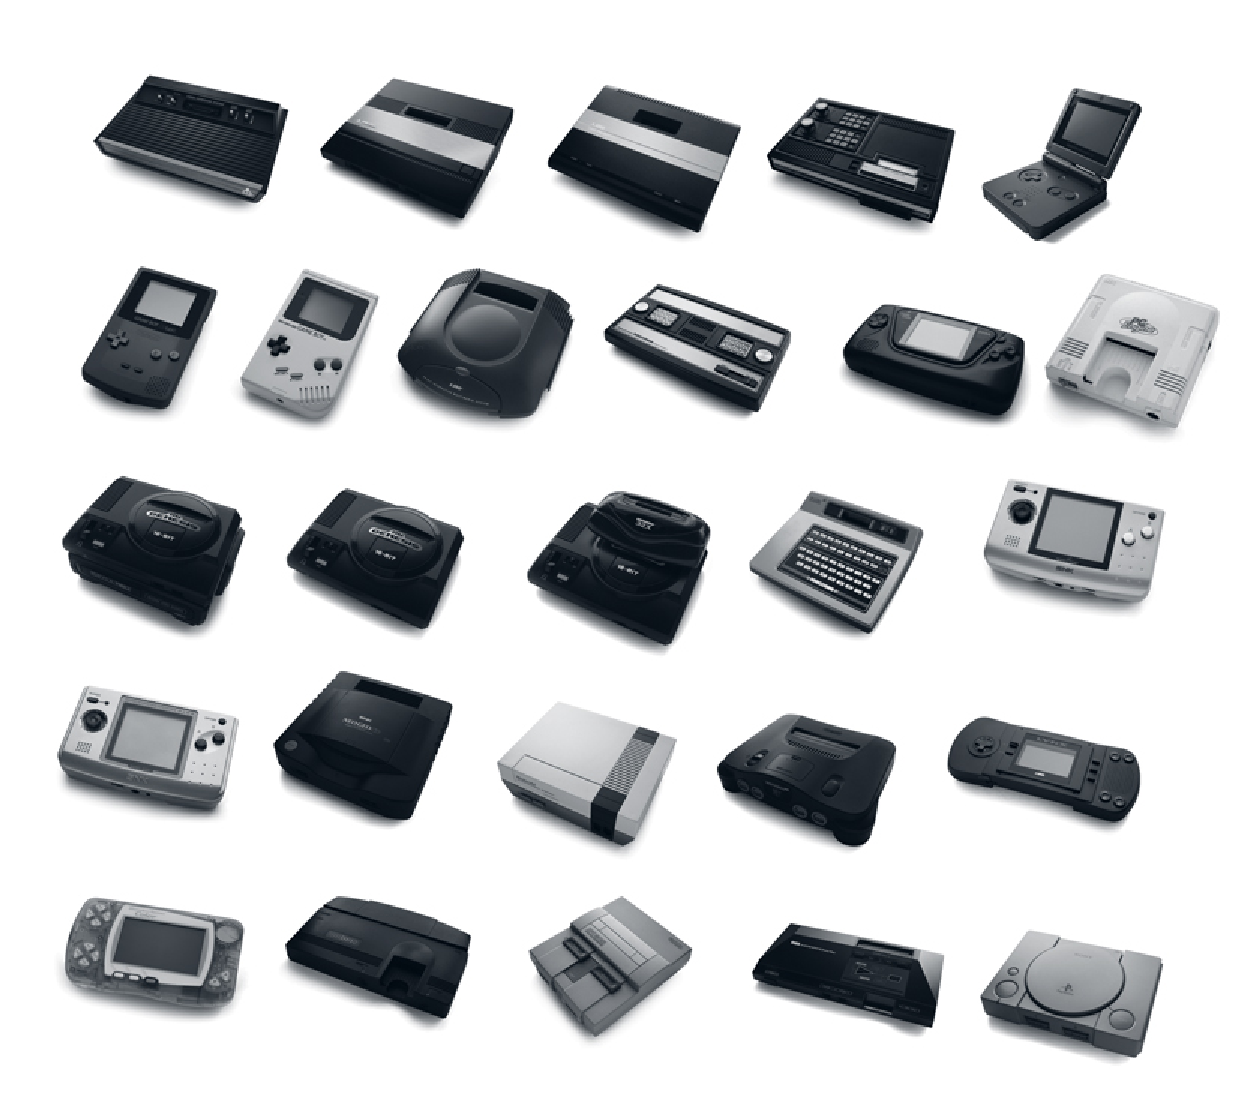
\epsfig{file=classicconsoles.eps,scale=0.5}
\caption{A number of classic video game consoles.}
\label{fig1}
\end{figure}

To be perfectly honest, I have rarely had quite as much fun with the games of today as I did back then.  Why is this?  Modern games certainly look prettier.  They are also way more technologically advanced.  So again, why is this?

\section{Features of Classic Video Game Consoles}
\begin{itemize}
\item{Cartridge-based}
\item{Typically between 8- and 32-bit graphics}
\item{3D titles were a rarity in all but the last few consoles.}
\end{itemize}

Table \ref{table1} shows a few historical facts about classic video game consoles.
\begin{table}
\centering
\caption{Timeline of interesting classic console facts.}
\label{table1}
\begin{tabular}{cl}
\hline
Year & Fact \\
\hline
1972 & The first video game console, the Magnavox Odyssey, was released. \\
1977 & The Atari 2600, one of the most well-known of the early video \\
& game consoles, was released. \\
1983 & The Nintendo Entertainment System, or NES, was released. \\
1990 & 30\% of Americans households owned the NES, compared to 23\% for \\
& all personal computers. \\
1994 & The Sony Playstation was released, signalling the beginning of \\
& the end for non-portable cartridge-based systems. \\
\hline
\end{tabular}
\end{table}
\end{document}

